\section{Experiment Results} \label{sec:exp-results}
The following table shows the results for each algorithm on each data set after running 10-fold cross validation.
Appendix \ref{app:conf-matrix} shows the detailed confusion matrix for each run.

Figure \ref{fig:performance-histogram} shows a comparison of each algorithm for the primary metric: macro-average.

\begin{center} \label{tb:cancer-dataset}
	\begin{tabularx}{\textwidth}{s | *5{>{\centering\arraybackslash}X}}
    \hline
    \textit{Algorithm} & \textit{Macro-Avg} & \textit{Precision} &  \textit{Accuracy} & \textit{F1-Score} \\ 
    \hline
    \multicolumn{5}{ c }{\textsc{Breast Cancer Data Set}} \\
    \hline
    K-NN & 0.801     &     0.903    &      0.859      &    0.849      \\
    NB &  0.929      &    0.910     &     0.923      &    0.919      \\
    TAN & 0.956      &    0.940    &      0.951    &      0.948         \\
    ID3 & 0.936     &     0.933     &     0.941       &   0.935   \\
	\end{tabularx}
\end{center}
\begin{center} \label{tb:glass-dataset}
	\begin{tabularx}{\textwidth}{s | *5{>{\centering\arraybackslash}X}}
    \multicolumn{5}{ c }{\textsc{Glass Data Set}} \\
    \hline
    K-NN & 0.865     &     0.946     &     0.973    &      0.904    \\
    NB &  0.257      &    0.216       &   0.790      &    0.235    \\
    TAN & 0.317    &      0.361     &     0.803      &    0.338   \\
    ID3 & 0.943      &    0.950     &     0.989     &     0.946       \\
	\end{tabularx}
\end{center}
\begin{center} \label{tb:votes-dataset}
	\begin{tabularx}{\textwidth}{s | *5{>{\centering\arraybackslash}X}}
    \multicolumn{5}{ c }{\textsc{House Votes Data Set}} \\
    \hline
    K-NN & 0.907     &     0.891     &     0.900     &     0.899    \\
    NB &  0.500      &    0.310       &   0.621      &    0.383  \\
    TAN & 0.978     &     0.987     &     0.983      &    0.982         \\
    ID3 & 0.981    &      0.975     &     0.979     &     0.978    \\
	\end{tabularx}
\end{center}
\begin{center} \label{tb:iris-dataset}
	\begin{tabularx}{\textwidth}{s | *5{>{\centering\arraybackslash}X}}
    \multicolumn{5}{ c }{\textsc{Iris Data Set}} \\
    \hline
    K-NN & 0.933    &      0.935     &     0.956    &      0.934    \\
    NB &  0.167     &     0.178       &   0.444      &    0.172    \\
    TAN & 0.300    &      0.290      &    0.533     &     0.295     \\
    ID3 & 0.927    &      0.926     &     0.951     &     0.926      \\
	\end{tabularx}
\end{center}
\begin{center} \label{tb:soybean-dataset}
	\begin{tabularx}{\textwidth}{s | *5{>{\centering\arraybackslash}X}}
    \multicolumn{5}{ c }{\textsc{Soybean Data Set}} \\
    \hline
    K-NN & 1.000 & 1.000 & 1.000 & 1.000    \\
    NB &  0.500     &     0.281    &      0.787     &     0.360   \\
    TAN & 0.826     &     0.887     &     0.925     &     0.856  \\
    ID3 & 0.972     &     0.972    &      0.988     &     0.972      \\
	\end{tabularx}
\end{center}

\begin{figure}[!htb]
	\caption{Algorithm Performance}
    \centering
	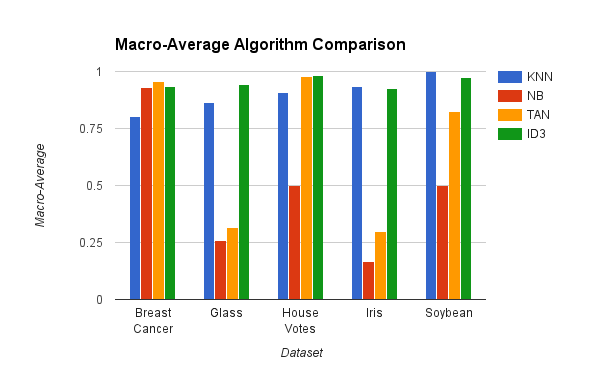
\includegraphics[width=\textwidth]{figures/performance-histogram.png}
    \label{fig:performance-histogram}
\end{figure}